\documentclass[11pt,a4paper]{article}
\usepackage[margin=0.9in]{geometry}
\usepackage[T1]{fontenc}
\usepackage[utf8]{inputenc}
\usepackage{graphicx}
\usepackage{hyperref}
\usepackage{enumitem}
\usepackage{float}
\usepackage{booktabs}

\title{Advanced Image Processing Methods\\Homework 6 Report}
\author{Peter Dobosi}
\date{\today}

\begin{document}
\maketitle

\section*{Goal}
Compare five pretrained YOLO26 sizes (\texttt{n}/\texttt{s}/\texttt{m}/\texttt{l}/\texttt{x}) on the African Wildlife dataset using \emph{inference only}---no training. For every model size, run \texttt{predict} on test images to inspect detections qualitatively, then run \texttt{val} on the official test split to obtain mAP at three IoU thresholds and wall-clock runtime, and contrast the trade-offs.

\section*{Method}
\begin{enumerate}[leftmargin=*,itemsep=1pt,topsep=2pt]
    \item \textbf{Data \& models.} The African Wildlife dataset has four classes (\texttt{buffalo}, \texttt{elephant}, \texttt{rhino}, \texttt{zebra}) split into 1052/225/227 train/val/test images; only the test split is touched. The five \texttt{yolo26\{n,s,m,l,x\}.pt} weight files supplied via Moodle are loaded as \texttt{ultralytics.YOLO} models without modification.

    \item \textbf{Inference (predict).} A fixed, seeded sample of 16 test images (the same set across all five models) is passed to \texttt{model.predict}. Per-image annotated frames with bounding boxes, class labels and confidence scores are rendered through Ultralytics' \texttt{Results.plot()} and saved as PNGs. The 16 frames are stitched into a $4\times4$ montage per model (Figure~\ref{fig:montage}).

    \item \textbf{Validation (val).} Each model is evaluated on the full 227-image test split via \texttt{model.val} with \texttt{split="test"}, recording \texttt{mAP@0.5}, \texttt{mAP@0.75}, \texttt{mAP@0.5:0.95}, and the wall-clock runtime measured around the call with \texttt{time.perf\_counter()}. Ultralytics also writes per-class P/R/F1/PR curves and a confusion matrix into the per-model run directory.

    \item \textbf{Environment.} A single shared virtualenv on Python~3.14.4 with \texttt{ultralytics 8.4.48}, \texttt{torch 2.11.0+cpu} and \texttt{torchvision 0.26.0+cpu}. All inference and validation runs were executed on CPU (no local GPU).
\end{enumerate}

\section*{Results}
\begin{table}[H]
    \centering
    \begin{tabular}{lcccc}
        \toprule
        Model & mAP@0.5 & mAP@0.75 & mAP@0.5:0.95 & Runtime (s) \\
        \midrule
        YOLO26-n & 0.962 & 0.918 & 0.840 & 13.95 \\
        YOLO26-s & 0.974 & 0.912 & 0.841 & 21.62 \\
        YOLO26-m & 0.968 & 0.912 & 0.830 & 56.50 \\
        YOLO26-l & 0.973 & 0.913 & 0.854 & 73.38 \\
        YOLO26-x & 0.974 & 0.927 & 0.847 & 154.02 \\
        \bottomrule
    \end{tabular}
    \caption{Test-split mAP and wall-clock runtime for the full 227-image \texttt{val} pass on CPU. Per-image inference times reported by Ultralytics scale similarly: 32~ms (\texttt{n}), 86~ms (\texttt{s}), 240~ms (\texttt{m}), 314~ms (\texttt{l}), 668~ms (\texttt{x}).}
    \label{tab:metrics}
\end{table}

All five models reach $\geq 0.96$ mAP@0.5 on this dataset; the largest spread across sizes is only $0.012$ at this threshold and $0.024$ at the much stricter mAP@0.5:0.95.

\section*{Analysis}
\textbf{How does performance change with model size?}
The mAP curves are essentially flat. From \texttt{n} to \texttt{x}, mAP@0.5 ranges in $[0.962, 0.974]$, mAP@0.75 in $[0.912, 0.927]$, and mAP@0.5:0.95 in $[0.830, 0.854]$. The progression is also non-monotonic: \texttt{m} is slightly worse than \texttt{s} on every metric, and \texttt{x} only narrowly tops \texttt{l}. With four well-separated, large-instance classes and only 227 test images, this benchmark effectively saturates already at the smallest model, and the residual differences sit within the noise of independently pretrained checkpoints on a small test set.

\textbf{Is there a point where a larger model no longer helps?}
Yes---right after \texttt{s}. The \texttt{n}$\rightarrow$\texttt{s} step is the only meaningful gain ($+0.012$ mAP@0.5) and costs a $\sim2.7\times$ slowdown. Every subsequent step (s$\rightarrow$m, m$\rightarrow$l, l$\rightarrow$x) costs another $\sim1.5$--$2\times$ in inference time but produces sub-percentage-point fluctuations in either direction. The plateau is most visible in mAP@0.5:0.95, where \texttt{l} (0.854) and \texttt{x} (0.847) are statistically indistinguishable from \texttt{n}/\texttt{s} (0.840/0.841).

\textbf{Best accuracy/speed compromise?}
\textbf{YOLO26-n} is the most defensible pick: 32~ms per image (5--21$\times$ faster than the larger sizes), only $1.2$~percentage points behind the best mAP@0.5 and $0.7$~pp behind the best mAP@0.5:0.95. If a slightly higher mAP@0.5 is preferred over peak throughput, \texttt{YOLO26-s} (0.974 mAP@0.5 at 86~ms/img) is the runner-up. The larger sizes are difficult to justify on this dataset.

\begin{figure}[H]
    \centering
    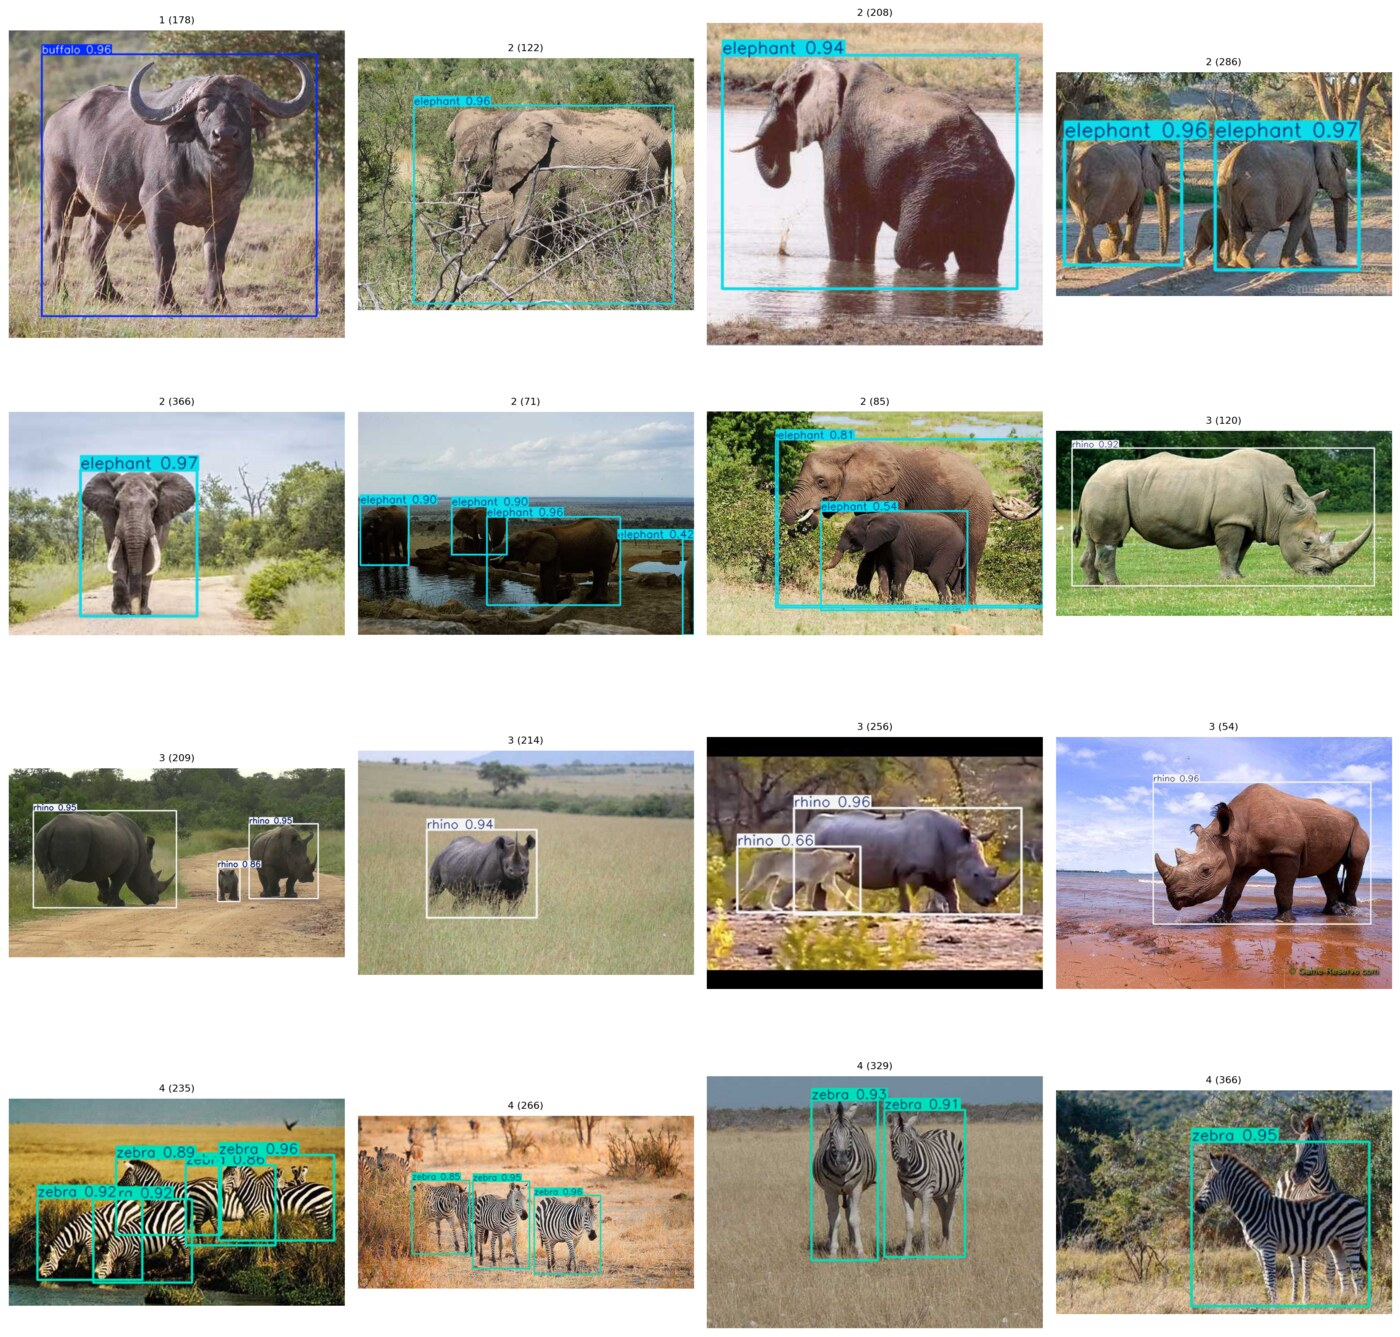
\includegraphics[width=0.62\textwidth]{output/report_figures/yolo26x_montage.jpg}
    \caption{$4\times4$ montage of YOLO26-x detections on the seeded test sample. All four classes are correctly localised and labelled with high confidence; the qualitative output is essentially indistinguishable from the smaller models, consistent with the saturation observed in Table~\ref{tab:metrics}.}
    \label{fig:montage}
\end{figure}

\end{document}
